\chapter{The Bias-Variance Tradeoff {\color{red} DRAFT} \label{chapter:biasvariance}}

In classification, \textbf{model complexity} (i.e. the effective number of parameters the model must fit) is typically related to the intricacy and complexity of the decision boundary; the more parameters in the model, the more complex the boundary.

\section{Goodness of Fit vs. Generalizability}

Training vs. test error

\section{Bias vs. Variance}

This figure shows the training and test error for KNN as a function of $K$ for a classification example similar to the one discussed in Chapter~\ref{chapter:classification}, as well as the training and test error for a linear model (which doesn't vary with $K$). You can see that the curves have characteristic shapes that vary with $K$. It turns out these shapes reflect a general principle for all supervised learning called the \textbf{bias-variance tradeoff}. 

The bias-variance tradeoff: KNN example. The Bayes error rate, or \textbf{irreducible error}, is the probability an instance is misclassified by a classifier that knows the true class probabilities given the predictors. From \emph{Elements of Statistical Learning}, Figure 2.4.

\begin{center}
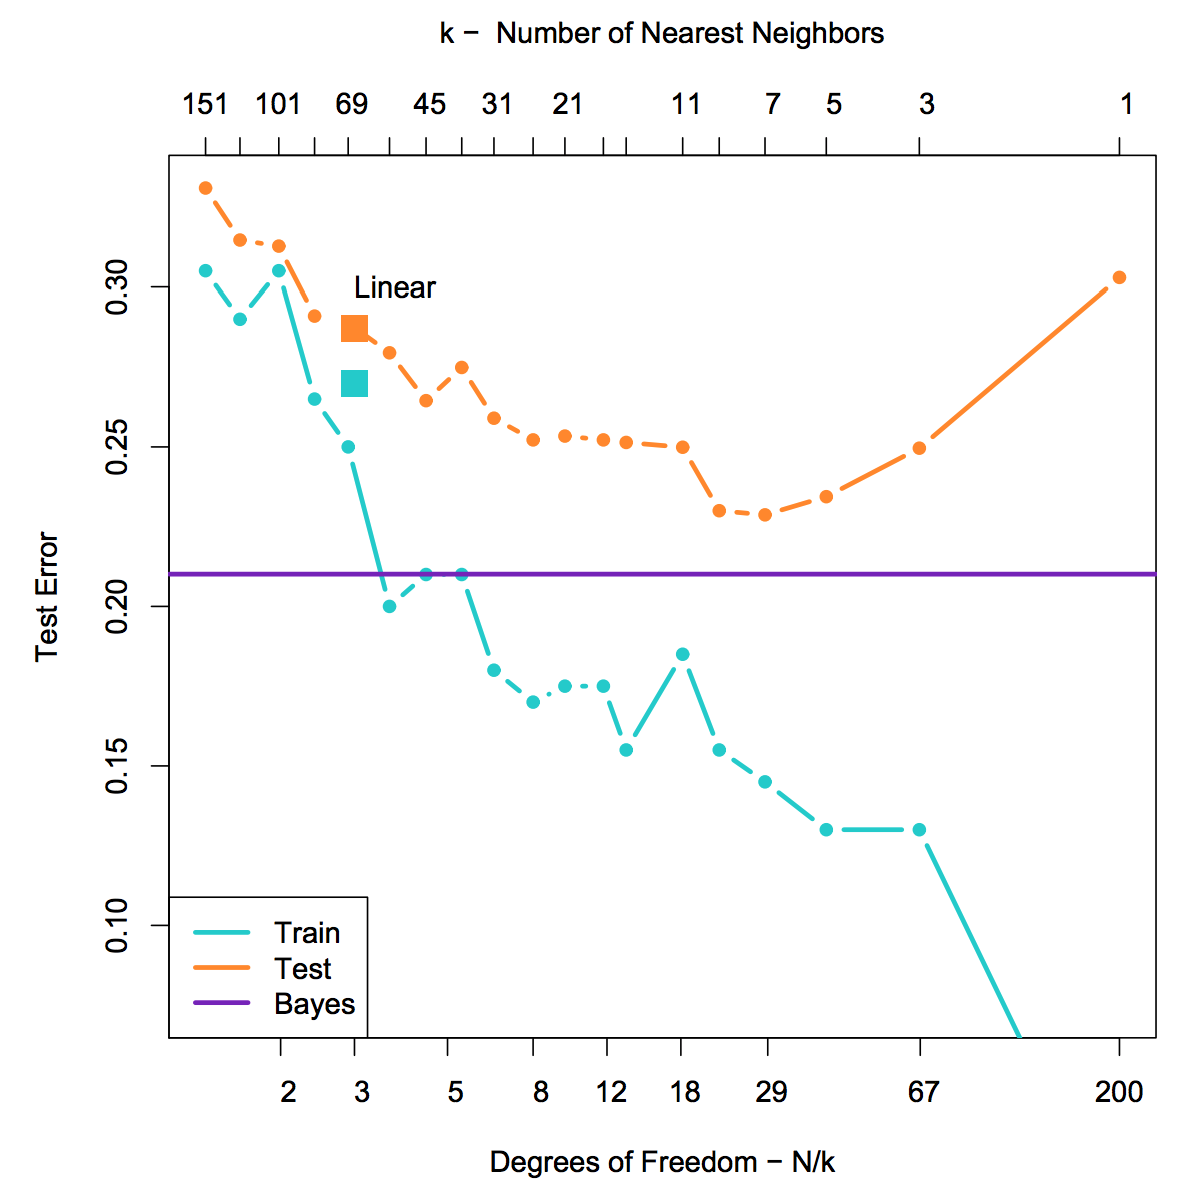
\includegraphics[width=0.8\textwidth]{img/l03-knn-linear-tradeoff.png}
\end{center}

Illustration of training vs. test error as a function of model complexity, as well as the bias-variance tradeoff. From \emph{Elements of Statistical Learning}, Figure 2.11.

\begin{center}
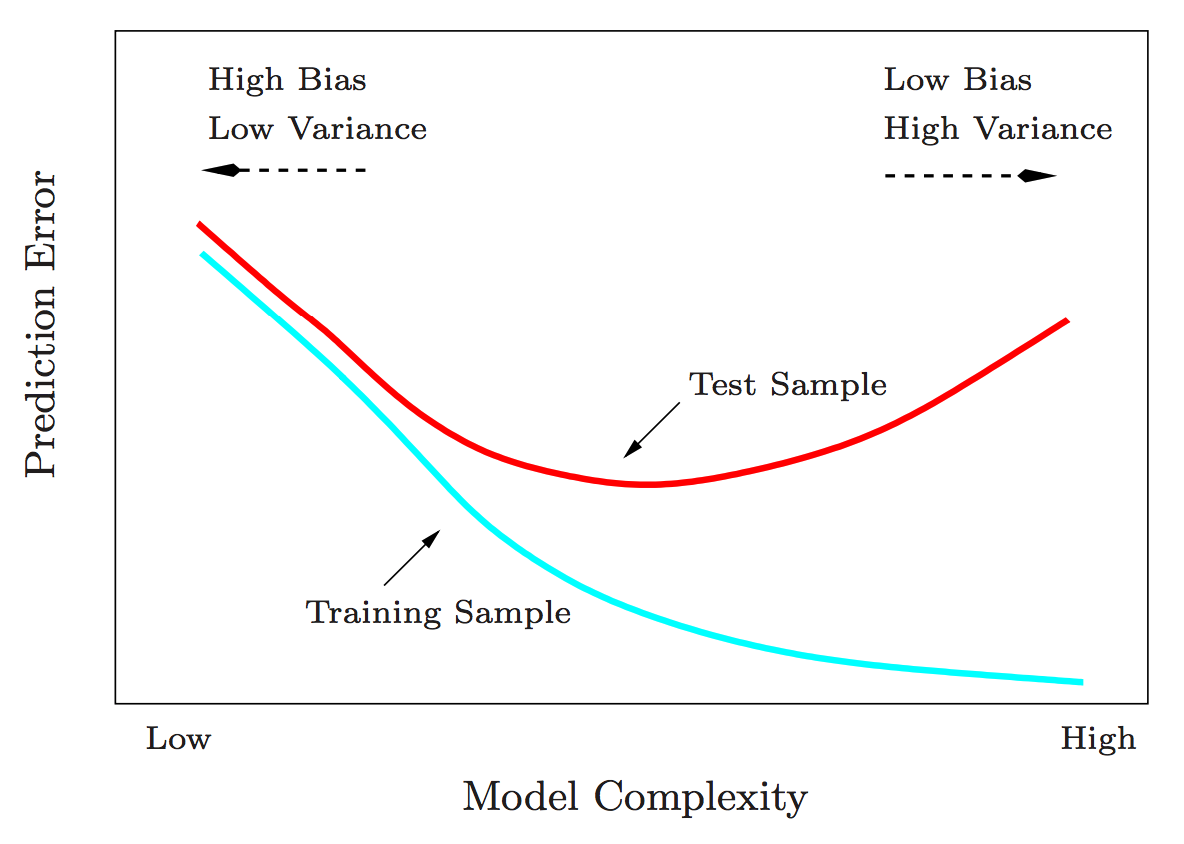
\includegraphics[width=0.8\textwidth]{img/l03-bias-variance-tradeoff.png}
\end{center}

A graphical illustration of the difference between bias and variance. Think of each dot as representing a single test example evaluated under the same model trained on slightly different datasets. The center of the target is the prediction the model should make for that test example. In the case of high bias and low variance, all of the models are off, but they are ``wrong in the same way''. If you average their predictions, the answer is still way off the mark. In the case of high variance, the models all make very different predictions on the same training example. However, their predictions are off in random directions from the center, so if you average their outputs, you'll get closer to the right answer. 

\begin{center}
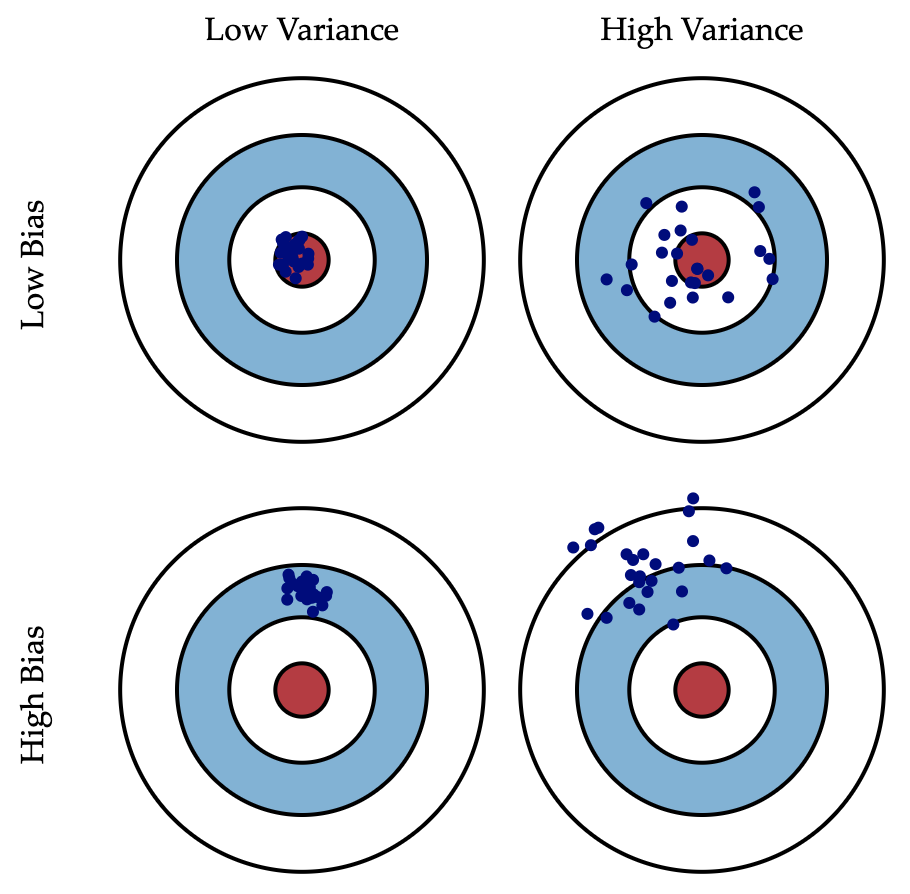
\includegraphics[width=0.7\textwidth]{img/targets-bias-variance.png}
\end{center}

\section{Overfitting vs. Underfitting}

\begin{question}{}
What are the advantages and disadvantages of KNN with low $K$ (e.g. $K=3$) vs. high $K$ (e.g. $K=50$)? The decision boundaries for the previous example with (left to right) $K=3, 15,$ and $50$ are shown below.
\begin{center}
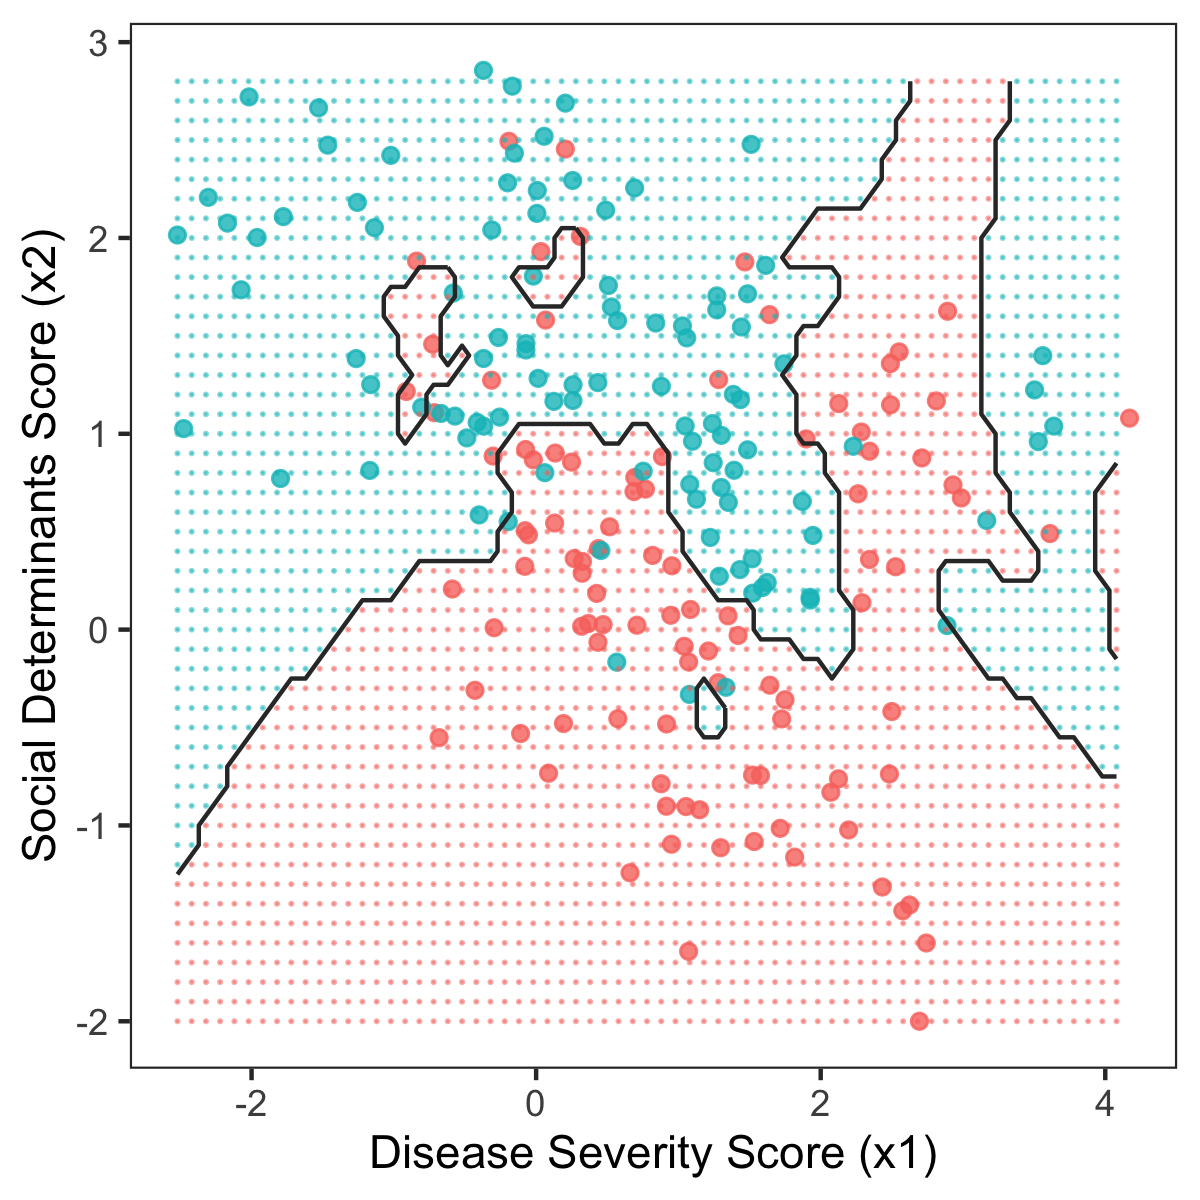
\includegraphics[width=0.3\textwidth]{img/esl-knn-3.png}
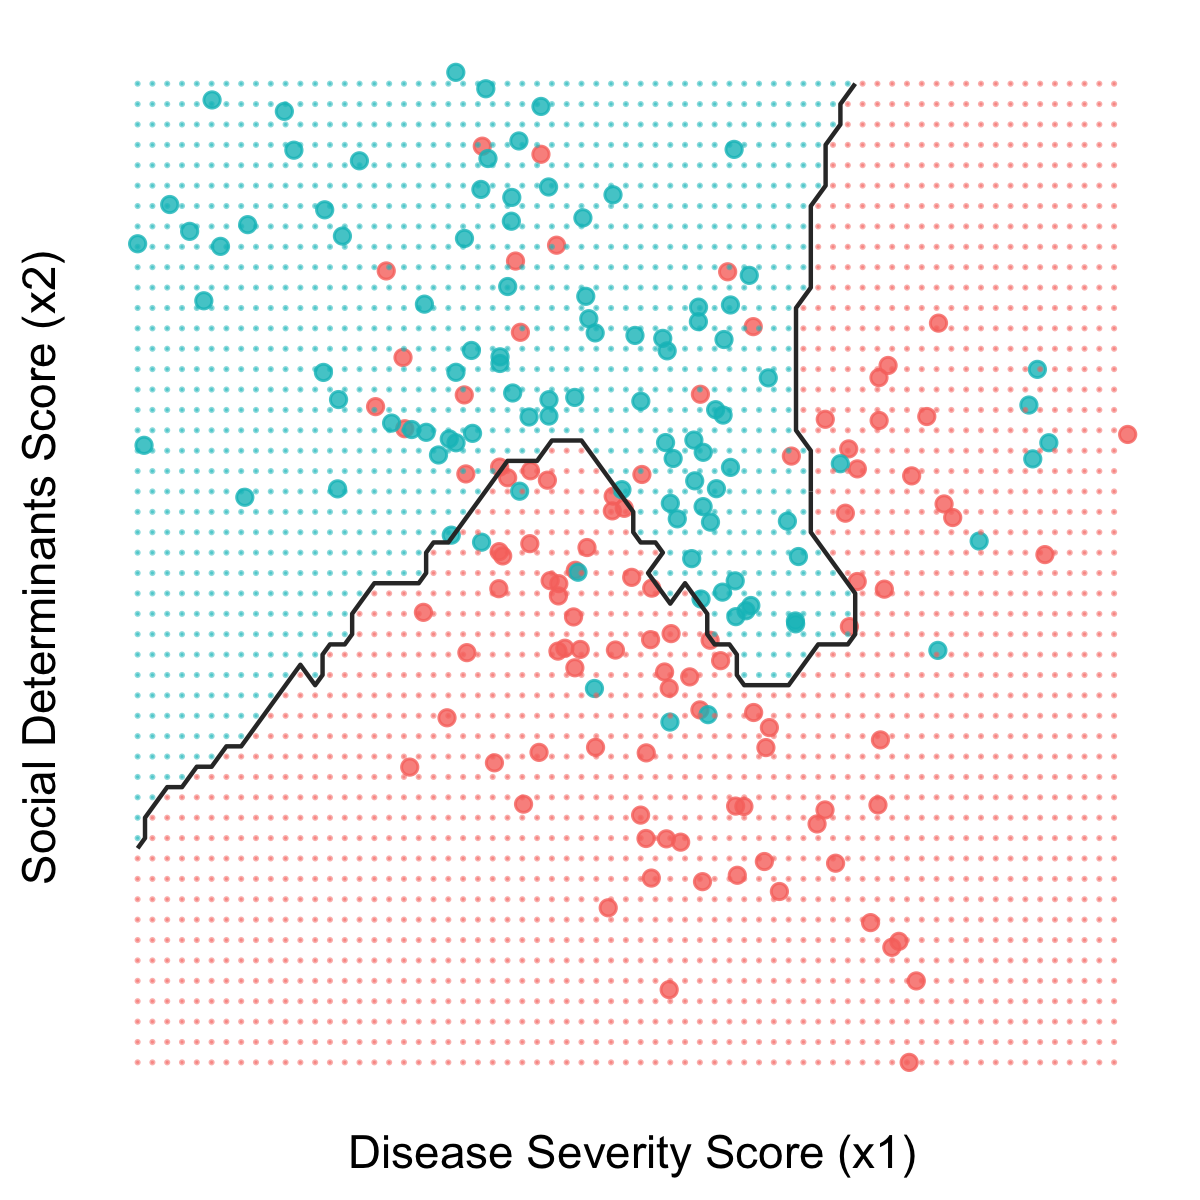
\includegraphics[width=0.3\textwidth]{img/esl-knn-15.png}
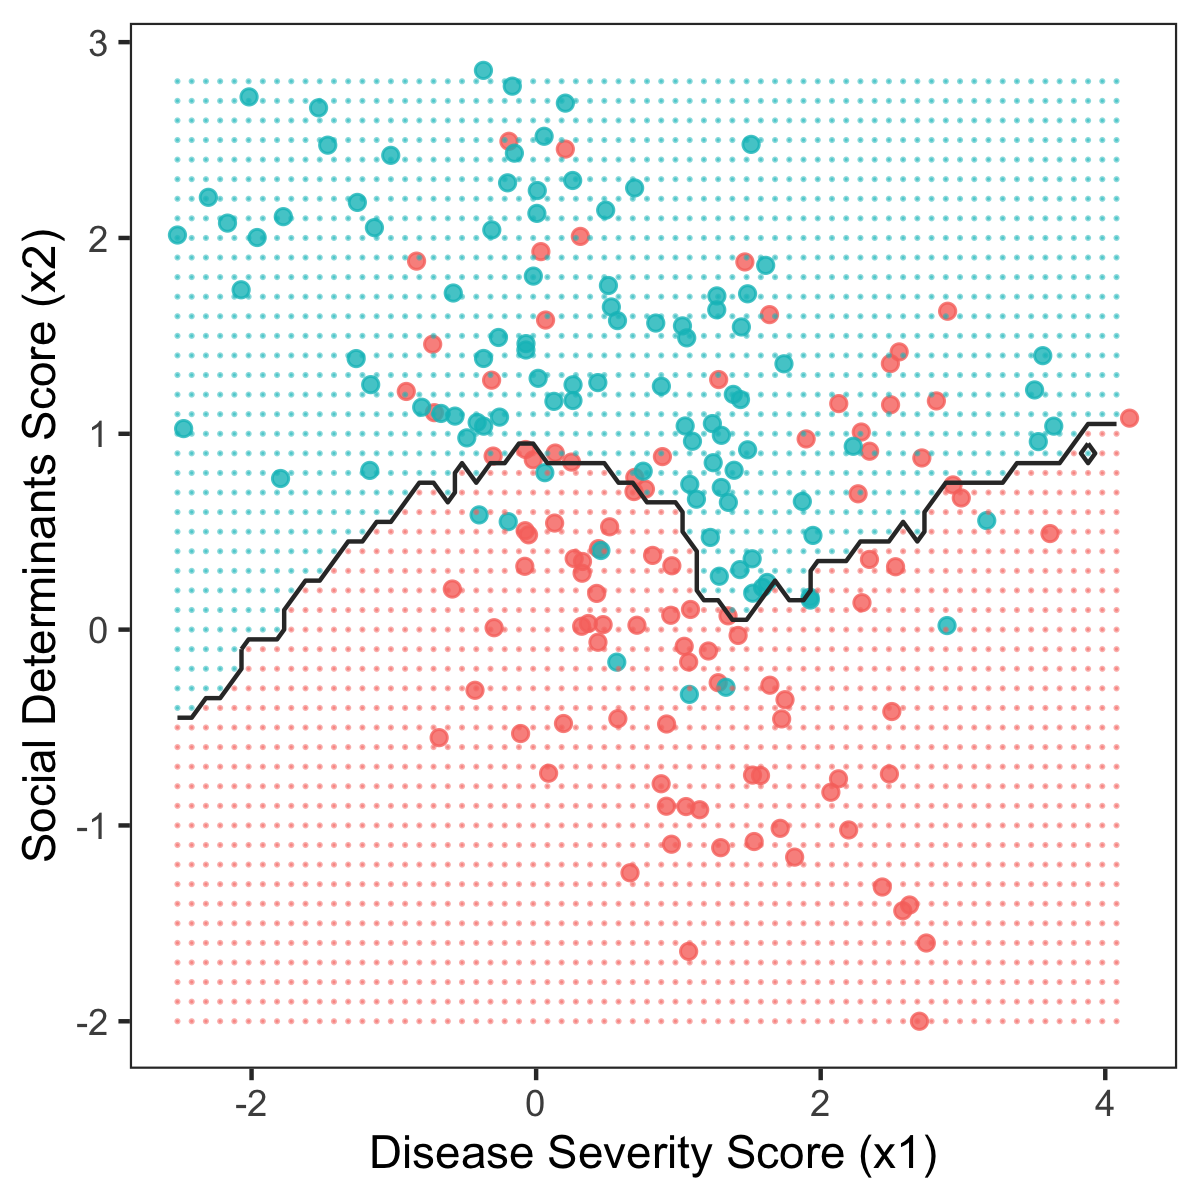
\includegraphics[width=0.3\textwidth]{img/esl-knn-50.png}
\end{center}
\end{question}

\begin{question}{}
We have discussed bias and variance in the context of classification (a yes/no outcome). How would training and test error, overfitting vs. underfitting, etc. be quantified if the outcome was a number, as in a regression problem (Chapter~\ref{chapter:regression})?
\end{question}
